\chapter{Evaluation of the Vision Pipeline}
\label{ch:cveval}

This chapter measures how well the pipeline detects people, classifies roles, finds interactions and how fast it runs. Every number names the report file it comes from; all files are in \path{backend/interaction/benchmarks/}. Numbers from clips the rules were tuned on are kept separate from numbers on held-out clips, and the headline result carries a confidence interval.

\section{Evaluation Method}
\subsection{Data}
Twenty-five labelled clips from one store and two cameras were split into two sets:
\begin{itemize}
\item \textbf{Tuning set} (11 clips, \path{benchmark.json}): 13 interactions and 4 pass-bys. The interaction rules were tuned on these clips, so their scores are optimistic.
\item \textbf{Held-out set B} (14 clips, \path{benchmark_set_b.json}): 17 interactions and 9 pass-bys. Set B uses only recordings from the detector's test and validation split, so no set-B frame was used to train the detector. It was looked at once during tuning, to set the rule that merges interaction spans separated by short gaps.
\end{itemize}
Labels were drawn and reviewed in CVAT. Every person in the 25 clips was reviewed for role (\path{persons.json}); a pipeline track takes the role of the reviewed person whose box it overlaps (IoU $\geq 0.3$ in at least half of its frames), which matched 109 of 113 tracks. The tuning-set labels have a single annotator.

\subsection{Metrics}
A predicted interaction matches a labelled one when their time spans overlap with temporal IoU $\geq 0.5$, one to one. Because this strict matching counts one long prediction that covers several short labels as both a miss and a false alarm, a per-second overlap score is reported as well. 95\,\% confidence intervals use a bootstrap over clips with 10\,000 resamples and a fixed seed~\cite{efron1979bootstrap}. Speed is the real-time factor: seconds of video processed per second of computation on a CPU.

\section{Results}
Table~\ref{tab:cv-results} gives the results with the fitted role weights adopted on 14 November 2026 (Section~\ref{sec:role-weights}). The headline is F1~0.450 on held-out set B, with a 95\,\% interval of 0.26--0.63; it meets the NFR-02 target of 0.40, although the lower end of the interval does not.

\begin{longtable}{P{0.19\textwidth}P{0.14\textwidth}P{0.26\textwidth}P{0.22\textwidth}P{0.11\textwidth}}
\caption{Vision pipeline results (fitted role weights unless stated)}\label{tab:cv-results}\\
\toprule
Stage & Metric & Set B (held out) & Tuning set & Source\\
\midrule
\endfirsthead
\toprule
Stage & Metric & Set B (held out) & Tuning set & Source\\
\midrule
\endhead
\bottomrule
\endfoot
Detector (best\_320, OpenVINO, 455 test images) & mAP50 / mAP50--95 / P / R & 0.969 / 0.896 / 0.963 / 0.953 & same detector & detector report\\
Interactions, proximity only & P / R / F1 & 0.346 / 0.529 / 0.419 (TP 9, FP 17, FN 8) & 0.619 / 1.000 / 0.765 & fitted reports\\
Interactions, with pose check & P / R / F1 & \textbf{0.391 / 0.529 / 0.450} (TP 9, FP 14, FN 8) & 0.765 / 1.000 / 0.867 (TP 13, FP 4, FN 0) & fitted reports\\
F1 95\,\% interval & with pose check & [0.261, 0.634] & [0.788, 0.960] & bootstrap\\
Per-second overlap & P / R / F1 & 0.521 / 0.943 / 0.671 & 0.711 / 0.904 / 0.796 & saved spans\\
Timing error & start / end (s) & 1.16 / 2.93 & 1.15 / 1.96 & reports\\
Roles & accuracy per track & 1.000 (56 tracks) & 0.957 (47 tracks) & fitted reports\\
Tracking & ID switches per minute & 1.68 & 2.04 & fitted reports\\
Speed & real-time factor (CPU) & \textbf{0.60$\times$} on an idle machine & & idle speed run\\
\end{longtable}

The fitted reports are \path{report_set_b_fitted_20261117.json} and \path{report_11_fitted_20261117.json}; the intervals are in \path{confidence_set_b_fitted_20261117.txt} and \path{confidence_11_fitted_20261117.txt}; the detector report is \path{report_set_b_merged.json} and the idle speed run is \path{report_set_b_speed_idle.json}. The per-second and timing rows come from the earlier run with hand-set role weights (\path{report_set_b_merged.json}, \path{report_11_merged.json}) and were not recomputed for the fitted run.

\paragraph{The pose check.} In the same run, the pose check removes 3 of the 17 proximity-only false positives on set B without losing a true positive, so precision rises from 0.346 to 0.391 and F1 from 0.419 to 0.450. On the tuning set it halves the false positives (8 to 4). Recall cannot change, because the check can only veto candidates.

\paragraph{Tuning set against held-out set.} F1 falls from 0.867 on the tuning clips to 0.450 on set B, and the two intervals do not overlap. This is the cost of tuning rules on a small set and the reason set B is the headline. The per-second recall of 0.943 on set B shows that most labelled interaction time is covered by some prediction: the pipeline usually finds the pair but draws the start and end differently from the labeller (Section~\ref{sec:cv-errors}).

\paragraph{Speed.} On an idle machine the pipeline processes set B at 0.60 times real time on a CPU (median 95\,ms per frame; the pose check costs 240--320\,ms per candidate pair), and up to about 1.5 times real time on individual clips. This meets NFR-01 (0.5 times real time). Runs that shared the CPU with other work measured 0.09--0.48 times and are not valid speed results. No GPU was available.

\section{Role Weights}
\label{sec:role-weights}
Each track's role is a weighted sum of employee evidence compared with a threshold. The original hand-set weights were reference similarity 0.55, bib colour 0.30, staff zone 0.10 and standing still 0.05, with a threshold of 0.45; on an uncalibrated camera the reference weight passes to the role detector's vote. A logistic regression with leave-one-clip-out validation was compared with them (Table~\ref{tab:roles}).

\begin{table}[H]
\centering
\caption{Hand-set against fitted role weights, leave-one-clip-out}\label{tab:roles}
\begin{tabular}{P{0.2\textwidth}P{0.15\textwidth}P{0.22\textwidth}P{0.13\textwidth}P{0.22\textwidth}}
\toprule
Set & Hand-set accuracy & Hand-set employee recall & Fitted accuracy & Source\\
\midrule
Tuning set (50 tracks) & 0.960 & 0.889 & 1.000 & \path{refit_benchmark/}\\
Set B (59 tracks) & 0.915 & 0.815 (misses 5 of 27) & 1.000 & \path{refit_benchmark_set_b/}\\
\bottomrule
\end{tabular}
\end{table}

The fit puts almost all weight on the role detector's vote (0.61) and bib colour (0.36), a little on standing still, and none on reference similarity or staff zones, with a threshold near 0.09 (\path{store_roles_fitted.json}). The zero weights mean those cues never occurred in the clips, because no camera is calibrated and no staff zone is drawn; they do not show the cues are useless. Figure~\ref{fig:role-sweep} shows that the fitted weights keep full employee recall over a wide range of thresholds, while the hand-set recall falls once the threshold passes about 0.2.

\begin{figure}[htbp]
\centering
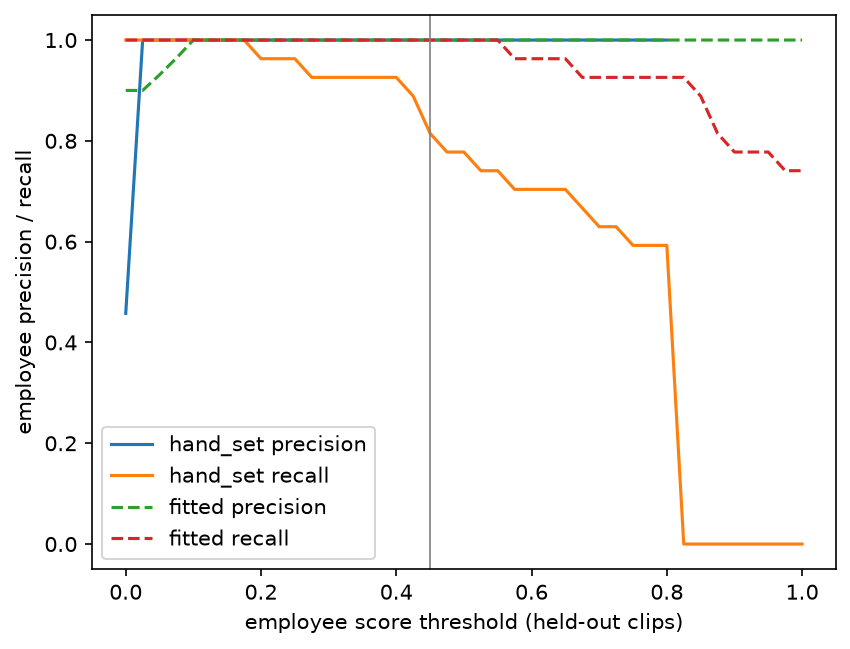
\includegraphics[width=0.62\textwidth]{ThesisFigs/role_threshold_sweep_set_b.png}
\caption[Role threshold sweep on held-out set B]{Employee precision and recall against the decision threshold on held-out set B: hand-set weights (solid) and fitted weights (dashed). The grey line is the hand-set threshold of 0.45.}
\label{fig:role-sweep}
\end{figure}

\textbf{Decision.} The fitted weights were adopted on 14 November 2026 and both benchmark specifications now load them for every clip. With them, role classification is correct for all 56 matched set-B tracks, meeting NFR-03. With two cameras and few clips this is not a general accuracy claim, and a store whose cameras are calibrated or have staff zones must refit the weights.

\section{Error Analysis}
\label{sec:cv-errors}
All false positives and misses on set B were inspected frame by frame (13 false positives and 8 misses in the hand-set run; the fitted run adds one false positive). They fall into three groups.
\begin{enumerate}
\item \textbf{Spans too long (4 false positives, 6 misses).} One prediction covers several shorter labelled interactions; on clip 155639 a prediction from 9.7 to 38.3\,s covers labels at 11.2--15.8, 19.5--28.4 and 34.3--36.7\,s. The 4\,s gap bridge joins what the labeller kept apart. The pair is found; the open question is whether a pause of 4--6\,s ends an interaction.
\item \textbf{Duplicates after a customer identity switch (4 false positives).} When the tracker gives a customer a new identifier mid-interaction, the merge cannot join the halves. The fix belongs in tracking, not in the merge rule.
\item \textbf{No label nearby (5 false positives).} Two look like missed labels (on IMG\_8838 part~2 the pair face each other for about 28\,s; on IMG\_8830 a customer gestures at a seated employee). One is two employees talking, and two are people side by side without engaging.
\end{enumerate}
If a blind re-check confirms the two suspected missed labels, set-B F1 would rise to about 0.49. Until that re-check is done, the reported figure is unchanged.

\section{Limitations}
\label{sec:cv-limits}
\begin{itemize}
\item \textbf{Small sample:} 30 labelled interactions in 25 clips from one store and two cameras; the interval on set-B F1 is wide (0.26--0.63).
\item \textbf{One look at set B} during tuning, to set the span merge.
\item \textbf{Identity switches} (1.7 per minute on set B) cause duplicate spans; no tracking fix has been made.
\item \textbf{Zone-level signals} (dwell per zone, entrance footfall, queues) are validated only on the synthetic fixture, because no camera has a registered map yet.
\item \textbf{Camera handoff} across cameras is implemented and unit-tested but not evaluated, because no crossings are labelled.
\item \textbf{Single annotator} for the tuning set; pass-bys are judgement calls.
\item \textbf{Detector scores} were not rerun with the fitted weights, because the detector test images are not on the evaluation machine; the detector is unchanged.
\end{itemize}
